\lecture[2022-05-17]{Course Overview}
\subsection{Overview}
\subsubsection{What is Data Science?}
``Data Science'' part of the course name. Fundamentally an interdisciplinary field - it is the application of data-centric, computational, and inferential thinking to understand the world (science) and solve problems (engineering).

Good data analysis is not just simply applying a statistics recipe or using a software. While there are many tools for data science, they are just tools - they do not do the important thinking.

\textbf{Example Questions in Data Science}

\begin{itemize}
\item What show should we recommend to our user to watch?
\item In which markets should we focus our advertising campaign?
\item Is the use of the COMPAS algorithm for prison sentencing fair?
\end{itemize}

\subsubsection{What will you learn in this class?}
``Principles and Techniques'' part of the course name. Course goals:
\begin{itemize}
\item \textbf{Prepare} students for advanced Berkeley courses in data management, ML, and statistics by providing the necessary foundation and context.
\item \textbf{Enable} students to start careers as data scientists by providing experience working with real-world data, tools, and techniques.
\item \textbf{Empower} students to apply computation and inferential thinking to address real-world problems.
\end{itemize}

\textbf{Topics Covered}

\begin{itemize}
\item \textbf{Data Analysis and Visualization}: Using NumPy, Pandas, visualization with matplotlib, Seaborn, plotly; Relational Databases and SQL, Regex
\item \textbf{Statistics}: Sampling, probability, and random variables.
\item \textbf{Machine Learning/Statistics Techniques}: Model designing/loss formulation, linear regression, feature engineering, regularization, bias-variance tradeoff, cross-validation; gradient descent, logistic regression; decision trees and random forests, PCA.
\end{itemize}

\subsection{Data Science Lifecycle}
High-level description of the data science workflow.
\begin{figure}[ht]
\begin{center}
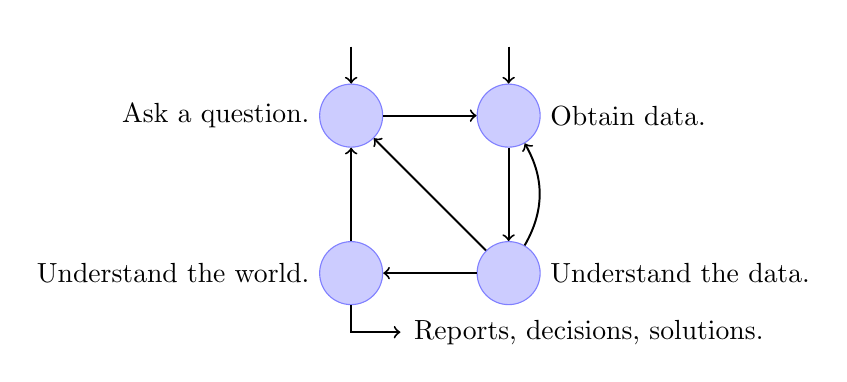
\begin{tikzpicture}
\node (aup) at (-1, 2) [draw=none] {};
\node (dup) at (1, 2) [draw=none] {}; 
\node (result) at (-0.25, -1.75) [draw=none, minimum size=0mm, label={[xshift=-2mm]right:Reports, decisions, solutions.}] {};
\node (ask) at (-1, 1) [circle, draw=blue!50, fill=blue!20, minimum size=8mm, label=left:Ask a question.] {};
\node (data) at (1, 1) [circle, draw=blue!50, fill=blue!20, minimum size=8mm, label=right:Obtain data.] {};
\node (uworld) at (-1, -1) [circle, draw=blue!50, fill=blue!20, minimum size=8mm, label=left:Understand the world.] {};
\node (udata) at (1, -1) [circle, draw=blue!50, fill=blue!20, minimum size=8mm, label=right:Understand the data.] {};
\draw [->, line width=0.25mm] (aup) edge (ask) (dup) edge (data) (ask) edge (data) (data) edge (udata) (udata) edge (uworld) (uworld) edge (ask) (udata) edge (ask);
\draw [->, bend right, line width=0.25mm] (udata) edge (data);
\draw [->, to path = (\tikztostart) |- (\tikztotarget), line width=0.25mm] (uworld) edge (result);
\end{tikzpicture}
\end{center}
\label{fig:ds-lifecycle}
\caption{Diagram of the data science lifecycle. Note the two different entry points.}
\end{figure}
\begin{enumerate}
\item \textbf{Question/Problem Formation} (Ask a question):
\begin{itemize}
\item What do we want to know?
\item What problems are we trying to solve?
\item What are the hypotheses we want to test?
\item What are our metrics for success?
\end{itemize}
\item \textbf{Data Acquisition and Cleaning} (Obtaining Data):
\begin{itemize}
\item What data do we have and what data do we need?
\item How will we sample more data?
\item Is our data representative of the population we want to study?
\end{itemize}
\item \textbf{Exploratory Analysis and Visualization} (Understand the Data):
\begin{itemize}
\item How is our data organized and what does it contain?
\item Do we already have relevant data?
\item What are the biases, anomalies, or other issues with the data?
\item How do we transform the data to enable effective analysis?
\end{itemize}
\item \textbf{Prediction and Inference} (Understand the World):
\begin{itemize}
\item What does the data say about the world?
\item Does it answer our questions or accurately solve the problem?
\item How robust are our conclusions and can we trust the predictions?
\end{itemize}
\end{enumerate}
\begin{example}[Demo: Data Science Lifecycle]{Begin with asking a question (step 1): Who are you?

Then gather and clean data (steps 2 and 3). Our population is Data 100 students, and some sub-questions could be \# of students, majors, year, diversity.

Focus on the final sub-question - diversity. Surveys of data scientists suggest that there are far fewer women:
\begin{center}
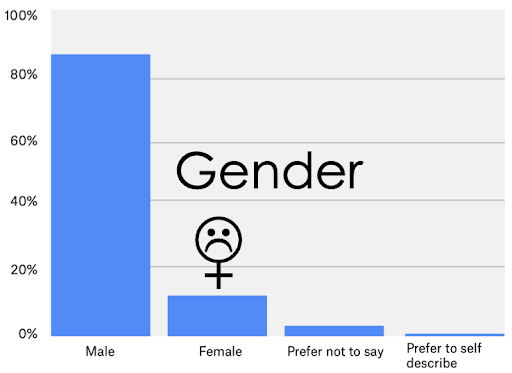
\includegraphics[width=0.6\textwidth]{diversitynt.png}
\end{center}

We want to see if this holds in the class (steps 4 and 1). We now have a new question: ``What fraction of students are female?'', and the process repeats itself again.

\tcbline

Now, since we want to find female students, a new question arises: ``Can we estimate a person's sex using their name?'' and we obtain more data: SSN baby names (steps 1, 2, and 3).

Using this data, we try to estimate the fraction of female students in the class (step 4). A possible classifier:
\begin{enumerate}
\item SSN: Proportion of female babies per name.
\item Use step 1 to classify each student name as F, M, or unknown.
\item Average step 2 to get the class proportion of females.
\end{enumerate}

However, the current model doesn't account for uncertainty. Create a new classifier:
\begin{enumerate}
\item SSN: Proportion of female babies per name.
\item For each student name from above:
\begin{enumerate}
\item Pick a number in $[0, 1)$.
\item If 2a is less than the SSN proportion (or 0.5 for Unknown), classify student as F; else M.
\end{enumerate}
\item Average step 2 to get a class proportion of females.
\end{enumerate}
\tcbline
\textbf{Recap}
\begin{itemize}
\item Find Data 100 data.
\item Explore interesting things about the class: names, majors, etc.
\begin{itemize}
\item Get stuck on a question: gender diversity.
\end{itemize}
\item Find more data: US SSN baby names.
\begin{itemize}
\item \textit{Approximate} gender with sex.
\end{itemize}
\item Create a classifier:
\begin{itemize}
\item Simple classifier: classifies names as exactly F/M.
\item Random classifier: all names have some probability of F.
\end{itemize}
\end{itemize}

\textbf{Limitations}
\begin{itemize}
\item US name data - while there are students from around the world here at Berkeley.
\item Names from since 1937; however, most students are born around 2000.
\item No ``rare'' names.
\item Sex as a proxy for gender - gender has been proxied to a binary classification.
\end{itemize}
Class data was \textit{fundamentally insufficent} to answer original question. Currently don't have the data to answer the question. Can survey the students to get the true proportion or use the data we have to get an estimate.
}
\end{example}
